%% LyX 2.1.1 created this file.  For more info, see http://www.lyx.org/.
%% Do not edit unless you really know what you are doing.
\documentclass[twocolumn,pre, reprint, nofootinbib]{revtex4-1}
\usepackage[latin9]{inputenc}
\setcounter{secnumdepth}{3}
\usepackage{amssymb}
\usepackage{graphicx}
\usepackage{amsmath}


\newcommand\blfootnote[1]{%
  \begingroup
  \renewcommand\thefootnote{}\footnote{#1}%
  \addtocounter{footnote}{-1}%
  \endgroup
}
\makeatletter

%%%%%%%%%%%%%%%%%%%%%%%%%%%%%% LyX specific LaTeX commands.
%% Because html converters don't know tabularnewline
\providecommand{\tabularnewline}{\\}

%%%%%%%%%%%%%%%%%%%%%%%%%%%%%% Textclass specific LaTeX commands.
% Fix a couple of bugs in REVTeX 4.1
\def\lovname{List of Videos}
\@ifundefined{textcolor}{}
{
 \definecolor{BLACK}{gray}{0}
 \definecolor{WHITE}{gray}{1}
 \definecolor{RED}{rgb}{1,0,0}
 \definecolor{GREEN}{rgb}{0,1,0}
 \definecolor{BLUE}{rgb}{0,0,1}
 \definecolor{CYAN}{cmyk}{1,0,0,0}
 \definecolor{MAGENTA}{cmyk}{0,1,0,0}
 \definecolor{YELLOW}{cmyk}{0,0,1,0}
}

\makeatother

\begin{document}

\title{Anti-ferromagnetic Ising Model in Hierarchical Networks }


\author{Xiang Cheng and Stefan Boettcher}

\affiliation{Department of Physics, Emory University, Atlanta, GA 30322, USA}
\begin{abstract}
The Ising antiferromagnet  is a convenient model of glassy dynamics.  It can introduce geometric frustrations and may give rise to a spin glass phase and glassy relaxation at low temperatures.  We apply the antiferromagnetic Ising model to 3 hierarchical networks which share features of both small world networks and regular lattices. Their recursive and fixed structures make them suitable for exact renormalization group analysis as well as numerical simulations. We first explore the dynamical behaviors using simulated annealing and discover an extremely slow relaxation at low temperatures. Then we employ the Wang-Landau algorithm to investigate the energy landscape and the corresponding equilibrium behaviors for different system sizes. Besides the Monte Carlo methods, renormalization group is used to study the equilibrium properties in the thermodynamic limit and to compare with the results from simulated annealing and Wang-Landau sampling. 
\smallskip 
\end{abstract}

\maketitle

\section{Introduction}

\label{sec:intro} 
BLANK

\section{RG Calculations}
\label{sec:RG}
 The setup of renormalization is started by separating the anti-ferromagnetic(AFM) Ising Hamiltonian into hierarchies
\begin{equation}
-\beta\mathcal{H} = \sum_{n=1}^{k-2} (-\beta \mathcal{H}_n)+ \mathcal{R}(K_2, K_3, \cdots)
\end{equation}
where $\mathcal{R}$ is the coupling beyond $\mathcal{H}_n$ of levels $k>2$. $\mathcal{H}_n$ depends on the interactions $K_0$ on the backbone and $L_0$, $L_1$, $K_1, \cdots$ among the long range couplings. We describe the RG procedure network by network. 












\subsection{RG Analysis of HN3 and HN5 without magnetic field}
\label{sec:HN35RG}

\subsubsection{RG setup and procedures}
For HN3 and HN5, the $\mathcal{H}_n$ for each hierarchy is
\begin{eqnarray}
\label{eq:z0}
 -\beta \mathcal{H}_n &=& K_0 \left(x_{n-2}x_{n-1} + x_{n-1}x_{n} +  x_{n}x_{n+1} +  x_{n+1}x_{n+2}\right) \nonumber \\ 
   && + K_1(x_{n-1}x_{n+1}) + L_0(x_{n-2}x_{n} + x_{n}x_{n+2}) \nonumber \\
   && + y L_1 (x_{n-2} x_{n+2})  + 4I 
\end{eqnarray}
where $y$ is 0 for HN3 and 1 for HN5. $I$ is a constant emerging since the first step of RG, and its initial value is 0. $L_0$ also stands for the coupling term emerged in the RG flow, and its initial value is also 0. The \underline{\emph{initial values}} for these parameters are
\begin{equation}
\begin{array}{l}
\displaystyle I = 0 \\
\displaystyle K_0 < 0 \\
\displaystyle K_1 < 0 \\
\displaystyle L_0 = 0 \\
\displaystyle L_1 < 0 \\
\end{array} 
\label{eq:init1}
\end{equation}
where $K_1$ is not changing in the RG flow because it is introduced again at every RG step. Therefore, it can be used as a reference of temperature. High temperatures $T \rightarrow \infty$ stands for $K_1\rightarrow -0$; while low temperatures $T\rightarrow 0$ corresponds to large $K_1 \rightarrow -\infty$.

After tracing the sites $x_{n-1}$ and $x_{n+1}$, in order to use RG, we have to get this form of equation
\begin{equation}
\label{eq:z1}
 -\beta \mathcal{H}_n = 2I' +  K'_0 \left(x_{n-2}x_{n} +  x_{n}x_{n+2}\right) + L'_0(x_{n-2}x_{n+2})
 \end{equation}
 which is `half' of original RG setup.
For convenience of the partition function and Mathematica calculation, we rewrite these parameters as
\begin{equation}
\begin{array}{l}
\displaystyle C = e^{-4I} = e^{-A[0]}  \\
\displaystyle \kappa = e^{-4K_0} = A[1] \\
\displaystyle \lambda = e^{-4L_0} = A[2] \\
\displaystyle \mu = e^{-2K_1} = e^{-2L_1} = A[3] 
\end{array} 
\label{eq:activities}
\end{equation}
The array $\{A[i]\}$ is used in the Mathematica calculations. The pre-factors of $K_0, K_1, I, {\rm and} L_1$ is for the convenience of the RG calculations. The reason to use exponential form for $C$ and $A[0]$ is to utilize more precision in Mathematica. Thus, the  \underline{\emph{initial values}}  for them are
\begin{equation}
\begin{array}{l}
\displaystyle C = 1, A[0]=0 \\
\displaystyle \kappa = A[1] = \mu^2 > 1\\
\displaystyle \lambda = A[2] =\mu^{2y} = 1\\
\displaystyle \mu = A[3] >1 \\
\end{array} 
\label{eq:init1}
\end{equation}
Generally, we only specify $\mu$ in the first step of RG; the initial values for HN3($y=0$) and HN5($y=1$) are determined by $\mu$ and $y$.

The relationship between $\mu$ and $T$ is the opposite as between temperature $T$  and $K_1$,  
\begin{equation}
\begin{array}{l}
\displaystyle T\rightarrow 0 \ \Leftrightarrow \ \ K_1 \rightarrow -\infty  \ \Leftrightarrow \ \ \mu \rightarrow \infty   \ \Leftrightarrow  \ \ {1}/{\mu}\rightarrow0\\
\displaystyle T\rightarrow \infty  \ \Leftrightarrow  \ K_1 \rightarrow -0 \ \Leftrightarrow  \ \ \mu \rightarrow 1 \  \ \Leftrightarrow  \ \  {1}/{\mu}\rightarrow 1 \\
\end{array} 
\label{eq:Ts}
\end{equation}
By tracing over all the $\{x_n\}$ in Eq. \ref{eq:z0} and Eq. \ref{eq:z1}, we can get equations and the following solutions
\begin{equation}
\begin{array}{l}
\displaystyle \kappa' = \frac{2\kappa \lambda (1+\mu) }{\kappa^2+2\mu \kappa +1} \\
\\
\displaystyle \lambda' = \mu^{2y} \frac{(1+\mu)(1+\kappa)^2}{2(\kappa^2+2\mu \kappa +1)}\\ \\
\displaystyle C' =  \frac{C^2 \kappa\mu}{\sqrt{2} (1+\kappa) (1+\mu)^{3/2}  \sqrt{ \kappa^2+2\mu \kappa +1}}   \\
\end{array} 
\label{eq:sol1}
\end{equation}

In Mathematica, what we get equivalently is actually
\begin{equation}
\begin{array}{l}

\displaystyle A'[1] = \frac{2A[1] A[2] (1+\mu) }{1+2\mu A[1] +A[1]^2} \\
\\
\displaystyle A'[2] = \mu^{2y}\frac{(1+\mu)(1+A[1])^2}{2(1+2\mu A[1]+A[1])}\\ \\ 
\displaystyle A'[0] =  \frac{1}{2} \log \left( \frac{e^{-4A[0]} \mu^2 A[1]^2}{2(1+\mu)^3 (1+A[1])^2 (1+2\mu A[1]+A[1]^2)}  \right) 
\end{array} 
\label{eq:activities}
\end{equation}

\subsubsection{Fixed point analysis}
For HN3 with $y=0$, we get 2 analytical fixed point solutions which are
\begin{equation}
\begin{array}{l}
\displaystyle \kappa = 1, \lambda =1;  \\
\displaystyle \kappa = 0, \lambda =\frac{1+\mu}{2} 
\end{array} 
\label{eq:fps3}
\end{equation}
where only the first one is a stable fixed point solution. The second one is only stable at infinitely high temperatures; any finite temperatures lead to the fixed point $\kappa =1, \lambda = 1.$ \\

For HN5 with $y=1$, the fixed points are more interesting. The fixed point solution are
\begin{equation}
\kappa = 0, \ \  \lambda = \mu^{2y}\frac{\mu+1}{2}
\label{eq:fps5}
\end{equation}

\begin{equation}
\kappa = \frac{1}{2}\left[\mu^2 -\mu + \sqrt{(\mu+1)(\mu^3 - 3\mu^2 +8\mu-4)} \right]
\label{eq:fps51}
\end{equation}
\begin{equation}
\lambda = \frac{\mu}{4}\left[\mu^2 -\mu+2 + \sqrt{(\mu+1)(\mu^3 - 3\mu^2 +8\mu-4)} \right]
\label{eq:fps52}
\end{equation}
For the parameter of interest $\kappa$, its solution Eq.\ref{eq:fps51} can be written in a general form as a function of $\mu$ ($\mu>1$)

\begin{eqnarray}
\kappa = \frac{1}{2}\Big[\sqrt{4\left( \mu^{1+y} + \mu^{y} - 1\right)+\left( \mu^{1+y} + \mu^{y} - 2\mu\right)^2}+ \nonumber \\
\mu^{1+y}+\mu^{y} -2\mu \Big] \nonumber \\
\label{eq:fyps_k}
\end{eqnarray}

The stability of the fixed points can be proved by both numerical iterations (Fig. \ref{fig:HN35KJ_ys}) and the eigvalue of the Jacobian below. 
\begin{equation}
J_{11} = \frac{\partial \kappa'(\kappa, \lambda)}{\partial \kappa}=-\frac{2 (\kappa -1) (\kappa +1) \lambda  (\mu +1)}{\left(\kappa ^2+2 \kappa  \mu +1\right)^2}
\end{equation}
\begin{equation}
J_{12} =  \frac{\partial \kappa'(\kappa, \lambda)}{\partial \lambda}= \frac{2 \kappa  (\mu +1)}{\kappa ^2+2 \kappa  \mu +1}
\end{equation}
\begin{equation}
J_{21} =\frac{\partial \lambda'(\kappa)}{\partial \kappa}=\frac{(\kappa -1) (\kappa +1) (\mu -1) (\mu +1) \mu ^{2 y}}{\left(\kappa ^2+2 \kappa  \mu +1\right)^2}
\end{equation}
\begin{equation}
J_{22} = \frac{\partial \lambda'(\kappa)}{\partial \lambda}=0
\end{equation}

The fixed point as a function of temperature ($\mu$ or $T$) at different $y$'s are shown in Fig. \ref{fig:HN35KJ_ys}.

\begin{figure}
\centering \includegraphics[width=0.8\columnwidth]{HN35_KJvsTys.pdf}
\protect\caption{The fixed point of $\kappa$ and corresponding $J$ using Eq. \ref{eq:fyps_k} for HN3, HN5, and their interpolations. $y=0$ corresponds to HN3; $y=1$ corresponds to HN5; and $y<0$ corresponds that the 'HN5' bonds are ferromagnetic;. In AF model, our temperature parameter $\mu$ is greater than 1. In this case, $1/\mu = 0 \Leftrightarrow T = 0$; $1/\mu = 1 \Leftrightarrow T\rightarrow \infty $. }
\label{fig:HN35KJ_ys} 
\end{figure}


$\kappa$ changes with $\mu$; the values of $\mu$ satisfying $\kappa(\mu)=0$ are likely to be the phase transition temperatures. After transformation of Eq.\ref{eq:fyps_k}, the equation $\kappa(\mu)=0$ can be rewritten as 
\begin{equation}
\mu^{1+y} + \mu^y -1 =0
\end{equation}
where there is a real root for $y<1.0$ in the antiferromagnetic range of $\mu>1$.  The transition temperature ($\mu_C$ or $T_C$) as a function of $y$ is shown in Fig.  \ref{fig:hn35transys}

\begin{figure}
\centering \includegraphics[width=0.6\columnwidth]{HN35ysTransVsY.pdf}
\protect\caption{Transition temperatures at different $y$'s. }
\label{fig:hn35transys} 
\end{figure}





\subsection{RG Analysis of HNNP}
\label{sec:HNNPRG}

\subsubsection{RG setup and procedures}
For HNNP, the $\mathcal{H}_n$ for each hierarchy is 
\begin{eqnarray}
\label{eq:hnnpz0}
 -\beta \mathcal{H}_n &=& K_0 \left(x_{n-2}x_{n-1} + x_{n-1}x_{n} +  x_{n}x_{n+1} +  x_{n+1}x_{n+2}\right) \nonumber \\ 
   && + K_1(x_{n-2}x_{n+1} + x_{n-1}x_{n+2})  \nonumber \\
   && +L_0(x_{n-2}x_{n} + x_{n}x_{n+2})  + 4I 
\end{eqnarray}
I is a constant parameter emerging after the first step of RG, and its initial value is 0. $L_0$ also stands for the coupling term emerged in the RG process, and its initial value is also 0. All the initials values for these activity parameters are
\begin{equation}
\begin{array}{l}
\displaystyle I = 0 \\
\displaystyle K_0 < 0 \\
\displaystyle K_1 < 0 \\
\displaystyle L_0 = 0 \\
%\displaystyle L_1 < 0 \\
\end{array} 
\label{eq:hnnpinit1}
\end{equation}
where $K_1$ is not changing in the RG flow because it is introduced `freshly' at every RG step. Therefore, it can be used as a reference of temperature. High temperatures $T \rightarrow \infty$ stands for $K_1\rightarrow -0$; while low temperatures $T\rightarrow 0$ corresponds to large $K_1 \rightarrow -\infty$.

The renormalization trace the sites $x_n$ and $x_{n+1}$ to get the renormalized form
\begin{equation}
\label{eq:hnnpz1}
 -\beta \mathcal{H}_n = 2I' +  K'_0 \left(x_{n-2}x_{n} +  x_{n}x_{n+2}\right) + L'_0(x_{n-2}x_{n+2})
 \end{equation}
 which is the same as that in HN3 and HN5. 
 \begin{equation}
\begin{array}{l}
\displaystyle C = e^{-4I} = e^{-A[0]}  \\
\displaystyle \kappa = e^{-4K_0} = A[1] \\
\displaystyle \lambda = e^{-4L_0} = A[2] \\
\displaystyle \mu = e^{-2K_1} = A[3] 
\end{array} 
\label{eq:activities}
\end{equation}
where $A[i]$ are the variables used in Mathematica calculations. The corresponding initial values are
 \begin{equation}
\begin{array}{l}
\displaystyle C = 1, A[0]=0 \\
\displaystyle \kappa = A[1]=\mu^2 > 1\\
\displaystyle \lambda = A[2] = \mu^{2y}\\
\displaystyle \mu = A[3] > 1 \\
\end{array} 
\label{eq:hnnpinit2}
\end{equation}

For the convenience of understanding from the traditional Ising model setup, the relationship among $\kappa$, interaction constant $J$, temperature $T$, and $\mu$ is
\begin{equation}
\begin{array}{l}
J^{(0)} = -1,  \\ \\
T = 2/\log(\mu) \\ \\
J^{(n)} = -\frac{T}{4}\log\kappa^{(n)}\\
\end{array}
\end{equation} 

In the calculation, we only need to specify the temperature $\mu$, then other initial values are determined accordingly.
The relationship between $\mu$ and $T$ is,  
\begin{equation}
\begin{array}{l}
\displaystyle T\rightarrow 0 \ \Leftrightarrow \ \ K_1 \rightarrow -\infty  \ \Leftrightarrow \ \ \mu \rightarrow \infty   \ \Leftrightarrow  \ \ {1}/{\mu}\rightarrow0\\
\displaystyle T\rightarrow \infty  \ \Leftrightarrow  \ K_1 \rightarrow -0 \ \Leftrightarrow  \ \ \mu \rightarrow 1 \  \ \Leftrightarrow  \ \  {1}/{\mu}\rightarrow 1 \\
\end{array} 
\label{eq:Ts}
\end{equation}
Eqs. \ref{eq:hnnpz0} and \ref{eq:hnnpz1} yields the RG recursions
\begin{equation}
\begin{array}{l}
\displaystyle \kappa' = \frac{\kappa \lambda (1+\mu)^2 }{(1+\mu\kappa)^2} \\
\\
\displaystyle \lambda' = \frac{(\kappa + \mu)^2} {(1 + \mu \kappa)^2} \\ \\
\displaystyle C' =  \frac{C^2 \kappa\mu^2} {(1+\mu)^2 (\kappa+\mu) (1+ \mu\kappa)}   \\
\end{array} 
\label{eq:hnnpsol1}
\end{equation}
These solutions are also the same as those in Ref. \cite{boettcher2011rg} since the setup is the same but the temperature domain $\mu$ is different.



\subsubsection{Fixed point analysis}

\begin{figure}[h!]
\centering 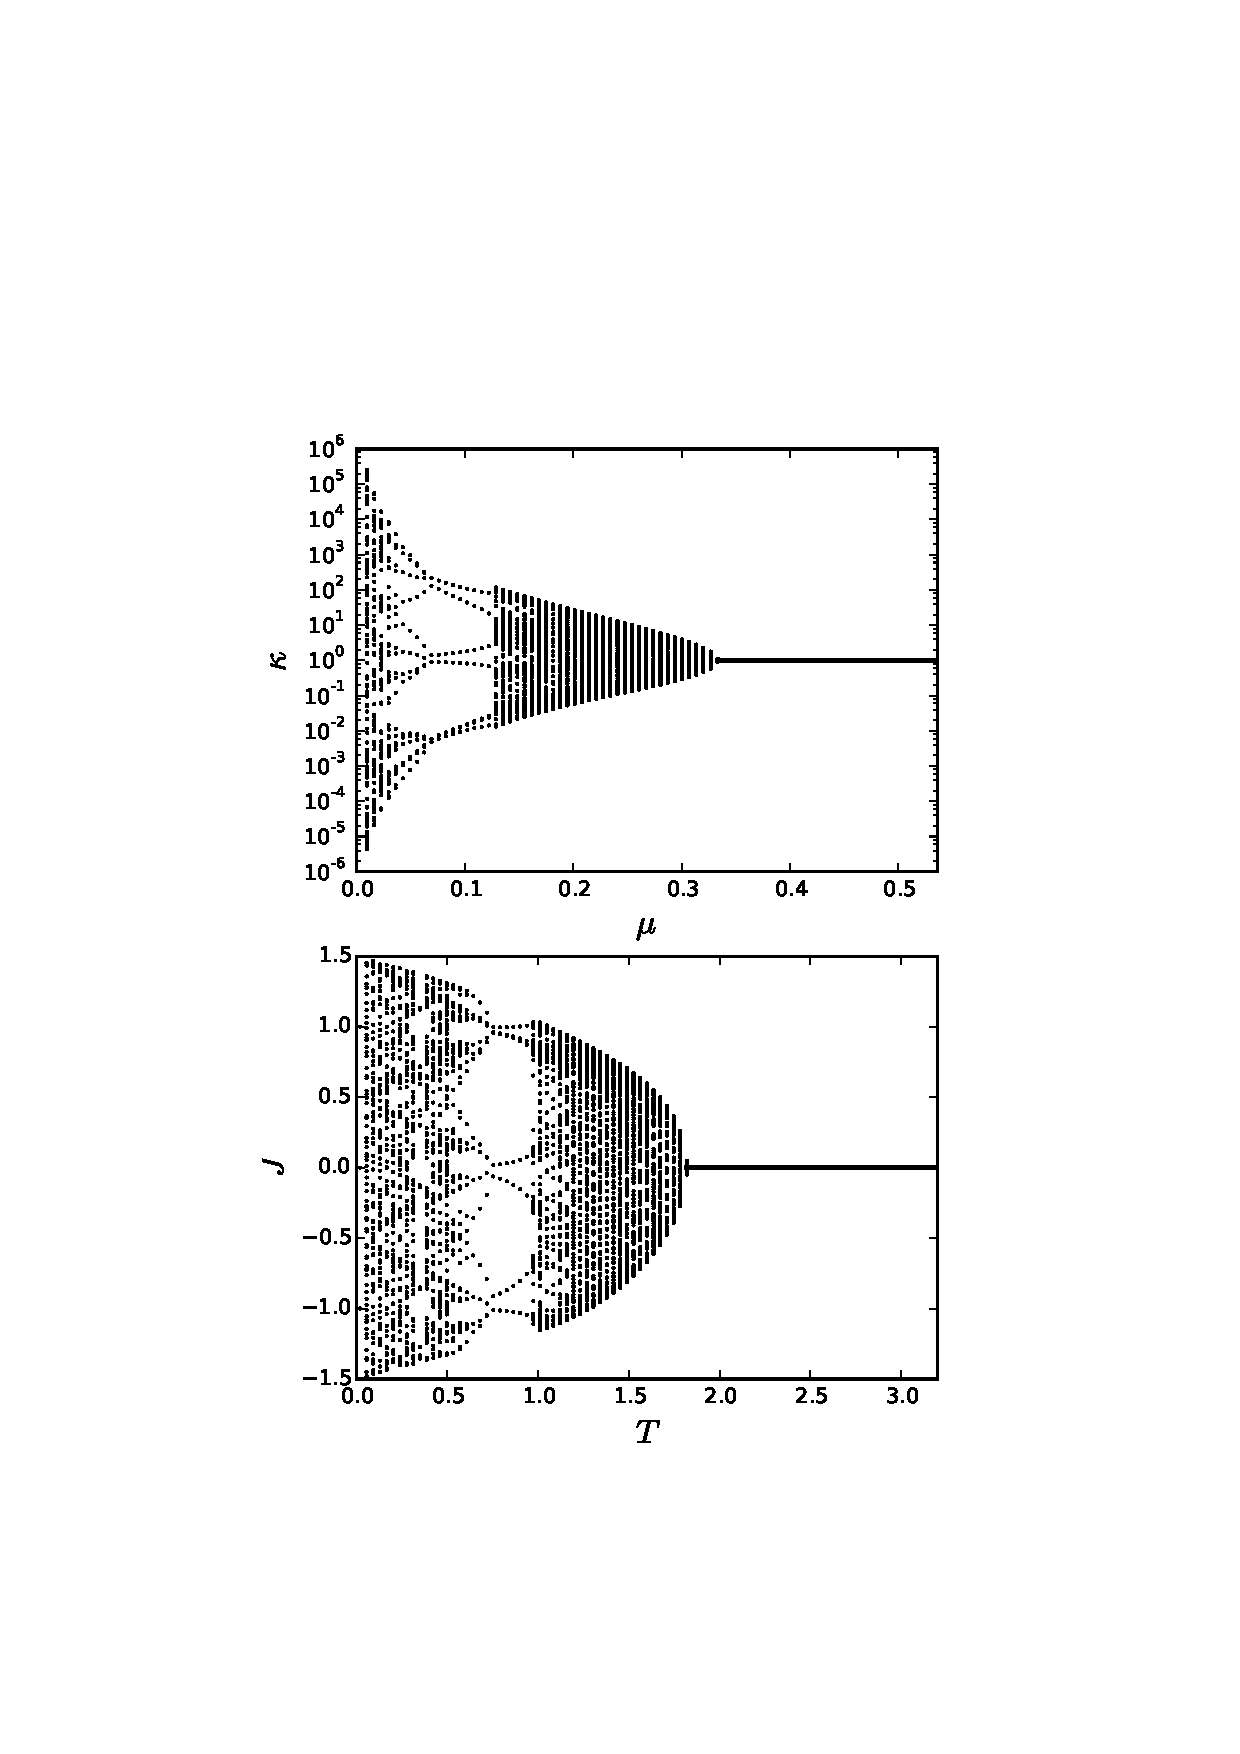
\includegraphics[width=0.9\columnwidth]{HNNP_RG_Kvsmu_JvsT.pdf}
\protect\caption{ $\kappa$ and $J$ of HNNP RG recrusive numerical results. When $1/\mu < 1/3$ or $T < 2/\log(3)$, there is no stable fixed point. }
\label{fig:hnnpkappa} 
\end{figure}

In the AFM scenario, for HNNP ($y = 0$), there are only 2 possible fixed points 
\begin{equation}
\begin{array}{l}
\kappa^* = 0, \ \lambda^* = \mu^2  \\ \\
\kappa^* = \lambda^* = 1 
\end{array}
\end{equation} 
 For HNNP, the actual fixed point is 1 for $\mu \le 3$ and {\it `oscillating fixed points' } for $\mu > 3$. This result is obtained from both numerical iterations of $\kappa*(\kappa, \lambda)$ and fixed point stability analysis from the Jacobian.

By simple numerial itertative calculation of Eq. \ref{eq:hnnpsol1}, we can get the data points of $\kappa$ as shown in Fig. \ref{fig:hnnpkappa}.



Another proof of the fixed point's unstability is the Jacobian matrix
\begin{equation}
J_{11} = \frac{\partial \kappa'(\kappa, \lambda)}{\partial \kappa}=\frac{\lambda  (\mu +1)^2}{(\kappa  \mu +1)^2}-\frac{2 \kappa  \lambda  \mu  (\mu +1)^2}{(\kappa  \mu +1)^3}
\end{equation}
\begin{equation}
J_{12} = \frac{\partial \kappa'(\kappa, \lambda)}{\partial \lambda}=\frac{\kappa  (\mu +1)^2}{(\kappa  \mu +1)^2}
\end{equation}
\begin{equation}
J_{21} = \frac{\partial \lambda'(\kappa)}{\partial \kappa}=\frac{2 (\kappa +\mu ) }{(\kappa  \mu +1)^2}-\frac{2 (\kappa +\mu )^2 \mu }{(\kappa  \mu +1)^3}
\end{equation}
\begin{equation}
J_{22} = \frac{\partial \lambda'(\kappa)}{\partial \lambda}=0
\end{equation}
The 2 eigenvalues are 
\begin{eqnarray}
Jevig = -\frac{(\mu +1)}{2 (\kappa  \mu +1)^3} \Big[\lambda  \mu  (\kappa +\kappa \mu -1)-\lambda \pm \nonumber \\ 
\sqrt{\lambda ^2 (\mu +1)^2 (\kappa  \mu -1)^2-8 \kappa  \left(\mu ^2-1\right) (\kappa +\mu ) (\kappa  \mu +1)} \Big] \nonumber \\
\end{eqnarray}

\begin{figure}[h!]
\centering \includegraphics[width=1.0\columnwidth]{HNNP_eigenvalues.pdf}
\protect\caption{The absolute values (1st norm) of the 2 complex eigenvalues for HNNP. For $0<\mu<1$, that is for the ferromagnetic case; while the antiferromagnetic region is $\mu>1$. You see the transition temperature is $\mu=3.0$ or $T=2/\log(3)=1.820478...$ because after that the $|eigenvalues|>1$ . }
\label{fig:hnnp_eigs} 
\end{figure}

We can plug in the 2 possible fixed points to these two eigenvalues, and the eigenvalues become
\begin{equation}
Jevig = \frac{\pm \sqrt{-7 \mu ^2-2 \mu +9}-\mu +1}{2 \mu +2}
\label{eq:hnnpJevig2}
\end{equation}
Because $\mu>1$, they are complex numbers. In this case, the absoluate values matter. As shown in Fig \ref{fig:hnnp_eigs}, by solving the Eq. \ref{eq:hnnpJevig2}$==1$, we can get the transition temperature is $\mu=3$.



\subsection{RG Analysis of HN6 and interpolations}
\label{sec:HPRG}

\subsubsection{RG setup and procedures}
For HN6, we can introduce another term with precoefficient $y$ in the $\mathcal{H}_n$ for each hierarchy
\begin{eqnarray}
 -\beta \mathcal{H}_n &=& K_0 \left(x_{n-2}x_{n-1} + x_{n-1}x_{n} +  x_{n}x_{n+1} +  x_{n+1}x_{n+2}\right) \nonumber \\ 
   && + K_1(x_{n-2}x_{n+1} + x_{n-1}x_{n+2}) + yL_1(x_{n-2} x_{n+2}) \nonumber \\
   && +L_0(x_{n-2}x_{n} + x_{n}x_{n+2})  + 4I 
\label{eq:hpz0}
\end{eqnarray}
$L_1$ is a new term to account for the extra links comparing to HNNP. $y=1$ is for HN6, and $y=0$ is for HNNP. We can tune $y$ continuously to explore the behaviors. All the initials values for these activity parameters are the same as in HNNP. The RG recursions are
\begin{equation}
\begin{array}{l}
\displaystyle \kappa' = \frac{\kappa \lambda (1+\mu)^2 }{(1+\mu\kappa)^2} \\
\\
\displaystyle \lambda' =\mu^{2y} \frac{(\kappa + \mu)^2} {(1 + \mu \kappa)^2} \\ \\
\displaystyle C' =  \frac{C^2 \kappa\mu^2} {(1+\mu)^2 (\kappa+\mu) (1+ \mu\kappa)}   \\
\end{array} 
\label{eq:hpsol1}
\end{equation}
These solutions are also the same as those in Ref. \cite{boettcher2011rg}.

\subsubsection{Fixed point analysis}

In this scenario, $y$ makes the fixed point much more complicated. One of the fixed point is
\begin{equation}
\kappa^* = 0, \ \ \lambda^* = \mu^{2+2y} 
\end{equation} 
Another positive fixed point for $\mu>1$ is 

\begin{equation}
\begin{array}{l}
\kappa^*=\frac{-2 \mu +\mu^{y/2}(\mu + 1) \left( \mu^{y/2}+\sqrt{4 (\mu -1) \mu +\mu ^y}\right) } {2 \mu ^2}  \\ \\
\lambda^* = \frac{1}{2} \mu ^{y-2} \left(2 (\mu -1) \mu +\mu ^y+\mu ^{y/2}\sqrt{4 (\mu -1) \mu +\mu ^y} \right) \\
\end{array}
\end{equation} 

Most interestingly, the fixed points are also chaotic for $-2<y<2$. When $y<-2$, the whole system became similar to ferromagnetic model; when $y>2$, other links is relatively weak, and the model becomes fairly simple and has no phase transition. Fig \ref{fig:hp6KJys}

\begin{figure*}
\centering \includegraphics[width=1.3\columnwidth]{HNP6_KvsMu_JvsT_ys3.pdf}
\protect\caption{Numerical calculation of $\kappa$ and $J$ at different $y$'s. As you may see, there is a chatoic transition for $-2.0<y<2.0$. For $y<-2.0$, there is a FM-like phase transition, and its transition temperature is shown in Fig.\ref{fig:hp6Tys}.}
\label{fig:hp6KJys} 
\end{figure*}

\begin{figure}
\centering \includegraphics[width=0.9\columnwidth]{HN6_TransTvsY1.pdf}
\protect\caption{Numerical Solution of chaotic transition temperature and phase transition temperature at different $y$'s for HNNP and HN6 interpolations. }
\label{fig:hp6Tys} 
\end{figure}

The chaotic transition temperature can be determined by the Jacobian matrix.
The Jocobian matrix
\begin{equation}
J_{11} = \frac{\partial \kappa'(\kappa, \lambda)}{\partial \kappa}=\frac{\lambda  (\mu +1)^2}{(\kappa  \mu +1)^2}-\frac{2 \kappa  \lambda  \mu  (\mu +1)^2}{(\kappa  \mu +1)^3}
\end{equation}

\begin{equation}
J_{12} = \frac{\partial \kappa'(\kappa, \lambda)}{\partial \lambda}=\frac{\kappa  (\mu +1)^2}{(\kappa  \mu +1)^2}
\end{equation}
\begin{equation}
J_{21} = \frac{\partial \lambda'(\kappa)}{\partial \kappa}=\frac{2 (\kappa +\mu ) \mu ^{2 y}}{(\kappa  \mu +1)^2}-\frac{2 (\kappa +\mu )^2 \mu ^{2 y+1}}{(\kappa  \mu +1)^3}
\end{equation}

\begin{equation}
J_{22} = \frac{\partial \lambda'(\kappa)}{\partial \lambda}=0
\end{equation}



The transition temperature can be solved by setting an equation of $|eigenvalue|==1$ because 
\begin{enumerate}
\item the eigenvalues are complex numbers, and the abs(eigenvalue) is the 1st norm; 
\item For complex eigenvalues, if the 1st norm is smaller than 1, the recursive equations can reach a stable fixed point; otherwise, it would not. Also, complex eigenvalues usually mean oscillating flow of the parameters, which is what we see in the numerical iterations.
\item The equation of the eigenvalue is very long, complex, and not solvable analytically. It is not shown here, but we can numerically solve it and find the chaotic transition temperature. The transition temperatures at different $y$ is shown in Fig. \ref{fig:hp6Tys}.
\end{enumerate}


When $y<-2.0$, we can have FM-like phase transition, and the transition temperature can obtained by solving $\kappa^*=0$. That is
\begin{equation}
1 - \mu^{1 + y} - \mu^{2 + y} = 0 
\end{equation}
The phase transition temperature is shown in the Fig. \ref{fig:hp6Tys}.



%\begin{figure*}
%\centering \includegraphics[width=2\columnwidth]{AFM_HN_ys_1okvsmu.pdf}
%\protect\caption{$1/\kappa$ vs $1/\mu$ calculating using Eq.\ref{eq:fps_k}. The black, red, and green vertical lines are from $y=-10, -2.0,\ {\rm and\ } -1.5$, respectively. They are due to the intersection of these curves and $\kappa = 0$. In AF model, $1/\mu = 0 \Leftrightarrow T = 0$; $1/\mu = 1 \Leftrightarrow T\rightarrow \infty $ }
%\label{fig:HN35_ys} 
%\end{figure*}
%\section*{Acknowledgements}
%We thank the U. S. National Science Foundation for its support through
%grant DMR-1207431.

\bibliographystyle{apsrev4-1}
%\bibliography{Jamming}
\bibliography{cheng}

\end{document}
